\documentclass{beamer}
%\documentclass[draft]{beamer}

\usepackage[utf8]{inputenc}
\usepackage[brazil]{babel}
\usepackage{ulem}				% traço sobre o texto
\usepackage{color}				% mudar com em texto
\usepackage{colortbl}			% adiciona cor a células nas tabelas
\usepackage{pgfpages}			% imprimir mais de um slide por página

%\pgfpagesuselayout{4 on 1}[a4paper,border shrink=5mm,landscape]

\setbeamertemplate{footline}[frame] %number]	% número de páginas nos slides
%\setbeamertemplate{navigation symbols}{}	% retirar barra de navegação

%\usetheme{Warsaw}
%\usetheme{Copenhagen}
\usecolortheme{whale}

\title{Coding Dojo de PHP}
\subtitle{treinando programação orientada a objetos no PHP}
\author[Fabrízio Mello]{Fabrízio de Royes Mello e Guilherme Silva de Lacerda}
\institute{\#guma10anos - Grupo de Usuários de Métodos Ágeis do RS\\
\url{http://codingbyexample.org}}
%\date{\today}
\date[guma10anos]{05 de abril de 2014}
\subject{tutorial}
\keywords{dojo, php, guma}
\logo{
\includegraphics[scale=0.2]{guma.jpg}}

\begin{document}

% criando a página de rosto
\begin{frame}
	\titlepage
\end{frame}


%%%%%%%%%%%%%%%%%%%%%%%%%%%%%%%%%%%%%%%%%%%%%%%%%%%%%%%%%%%%%%%%%%%%%%%%%%%%%%%
%%%%%%%%%%%%%%%%%%%%%%%%%%%%%%%%%%%%%%%%%%%%%%%%%%%%%%%%%%%%%%%%%%%%%%%%%%%%%%%

\begin{frame}
	\frametitle{Apresentação}
	\begin{block}{Fabrízio de Royes Mello}
		\begin{itemize}
			\item Especialista em Banco de Dados
			\item Colaborador Comunidade Brasileira de PostgreSQL
			\item Colaborador PostgreSQL Global Development Group
			\item @fabriziomello
		\end{itemize}
	\end{block}
	\begin{block}{Guilherme Silva de Lacerda}
		\begin{itemize}
			\item Especialista em Métodos Ágeis
			\item Agile Coach
			\item Colaborador GUMA/RS
			\item Professor Universitário
			\item @guilhermeslac
		\end{itemize}
	\end{block}
\end{frame}

\begin{frame}
	\frametitle{Sobre esta apresentação}
	\begin{itemize}
		\item esta apresentação está disponível em: \url{http://github.com/fabriziomello/guma10anos}
		\item esta apresentação está sob licença \textit{Creative Commons Atribuição 3.0 Brasil}: \url{http://creativecommons.org/licenses/by/3.0/br}
	\end{itemize}
\end{frame}

\begin{frame}
	\frametitle{Dojo (DO=caminho e JO=lugar)}
		\onslide<1->{
			\begin{center}
				\begin{figure}
					\scalebox{0.32}{
						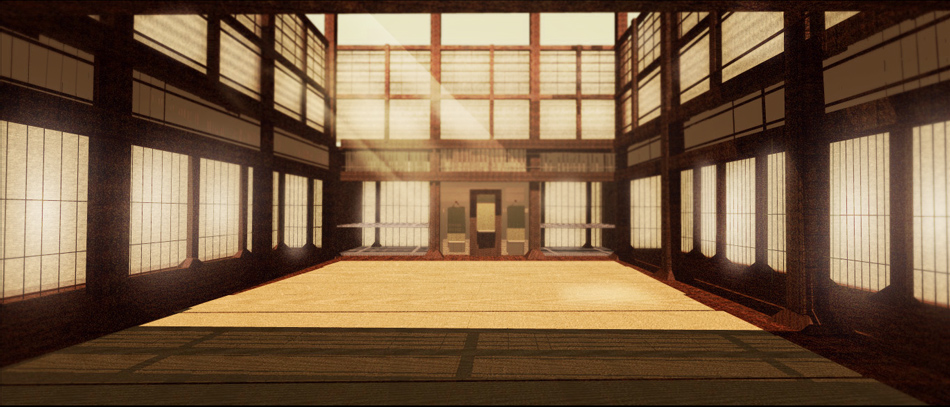
\includegraphics{dojo.jpg}
           			}
				\end{figure}
			\end{center}
		}
		"É o caminho da prática, a via do desenvolvimento integral, onde entramos em contato com o nosso melhor estado de ser."
\end{frame}

\begin{frame}
	\frametitle{Coding Dojo}
		\onslide<1->{
			\begin{center}
				\begin{figure}
					\scalebox{0.28}{
						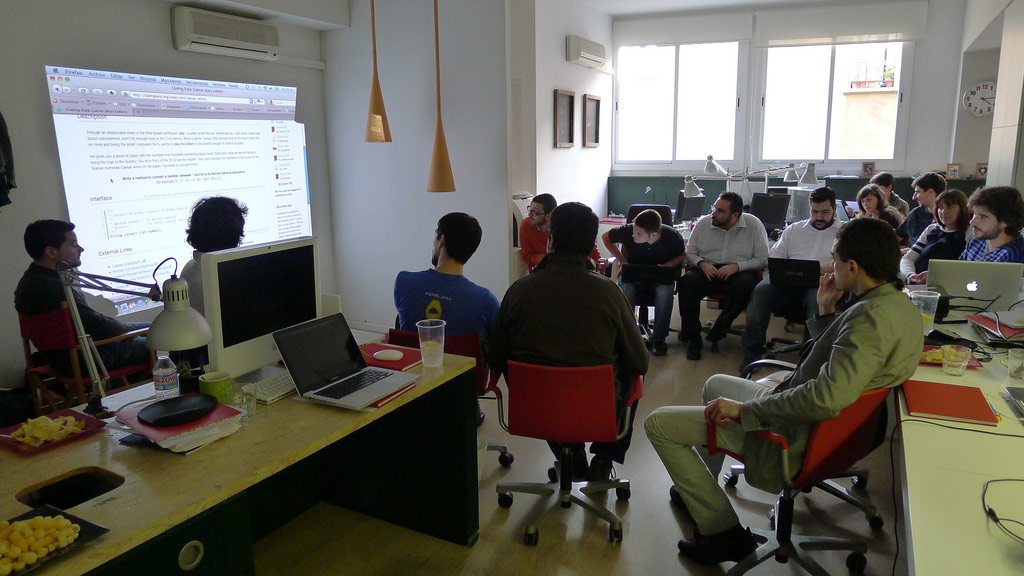
\includegraphics{coding_dojo.jpg}
           			}
				\end{figure}
			\end{center}
		}
\end{frame}

\begin{frame}
	\frametitle{Para que tudo isso?}
	\begin{itemize}
		\item ERRAR!!! Erro gera aprendizado
		\item Treinar as habilidades de programação
		\item Melhorar a comunicação
		\item Conhecer novas tecnologias
		\item Pensar "fora da caixinha"
		\item Diversão
	\end{itemize}
\end{frame}

\begin{frame}
	\frametitle{Cifra de César}
		\onslide<1->{
			\begin{center}
				\begin{figure}
					\scalebox{0.5}{
						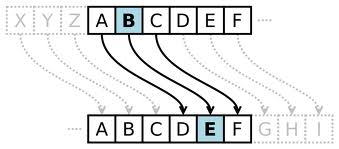
\includegraphics{cifra_cesar.jpg}
           			}
				\end{figure}
			\end{center}
		}
	Em criptografia, a Cifra de César, também conhecida como cifra de troca, código de César ou troca de César, é uma das mais simples e conhecidas técnicas de criptografia. É um tipo de cifra de substituição na qual cada letra do texto é substituída por outra, que se apresenta no alfabeto abaixo dela um número fixo de vezes. Por exemplo, com uma troca de três posições, A seria substituído por D, B se tornaria E, e assim por diante.
\end{frame}

\begin{frame}
	\frametitle{Problema / Regras}
	\begin{itemize}
		\item Implementar, em PHP, classes/métodos para criptografar e descriptografar strings usando a técnica da Cifra de César.
		\item Vamos usar TDD (Test-Driven Development) usando o Framework de Testes PHPUnit (www.phpunit.de)
		\item A cada 5min faremos a troca do piloto e outra pessoa da platéia entra na rodada
	\end{itemize}
\end{frame}

\begin{frame}
	\frametitle{Documentação Apoio}
	\begin{itemize}
		\item
		\url{http://www.php.net/manual/en/}
		\item \url{http://phpunit.de/getting-started.html}
	\end{itemize}
\end{frame}

\begin{frame}
	\frametitle{Retrospectiva}
	\begin{itemize}
		\item Pontos Positivos?
		\item Pontos Negativos?
	\end{itemize}
\end{frame}

\begin{frame}
	\frametitle{Perguntas}

	\begin{center}
		\Huge Dúvidas ?
		\vspace{0.5cm}
		\normalsize
	\end{center}
\end{frame}

\end{document}
